\documentclass[tikz]{standalone}
\usepackage{pgfplots}
\pgfplotsset{compat=1.15}
\usepackage{mathrsfs}
\usetikzlibrary{arrows,calc}
\usepackage{tkz-euclide}
\pagestyle{empty}

\definecolor{AngleClr}{rgb}{0,0.39215686274509803,0}
\definecolor{ShapeClr}{rgb}{0.6,0.2,0}
\definecolor{BlueClr}{RGB}{13,93,184}

\begin{document}

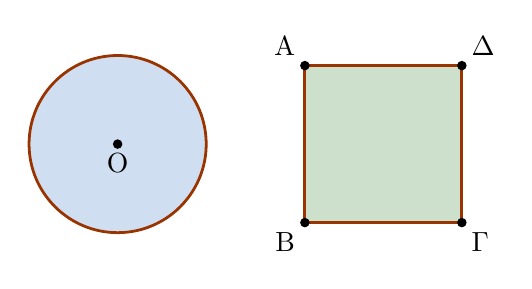
\begin{tikzpicture}[scale=.75]
\tkzSetUpLine[line width=1pt,color=black]
\tkzSetUpPoint[fill=black]

\tkzDefPoints{-1.5/0/O,0/0/X}
\newcommand{\Side}{1.32934}
\tkzDefPoints{3-\Side/\Side/A,3-\Side/-\Side/B,3+\Side/-\Side/C,3+\Side/\Side/D}

\tkzFillPolygon[fill=AngleClr,fill opacity=0.2](A,B,C,D)

\tkzDrawCircle[line width=1pt,color=ShapeClr,fill=BlueClr,fill opacity=0.2](O,X);

\tkzDrawPolygon[color=ShapeClr](A,B,C,D)

\tkzDrawPoints[size=3](A,B,C,D,O)


\tkzLabelPoint[above left](A){$\rm A$}
\tkzLabelPoint[below left](B){$\rm B$}
\tkzLabelPoint[below right](C){$\rm \Gamma$}
\tkzLabelPoint[above right](D){$\rm \Delta$}
\tkzLabelPoint[below](O){$\rm O$}

\end{tikzpicture}

\end{document}
